\section{Currency arbitrage}

\begin{tcolorbox}[width=\linewidth, sharp corners=all, colback=white!95!black]
    Consider the FX spot market, where we can see live exchange rates among several currencies (say USD, EUR, GBP, JPY, CHF, PLN, BRL, CNH). Design an algorithm that finds pure arbitrage opportunities on this market.
\end{tcolorbox}

Let's represent this market as a network where currencies are nodes and available exchange rates are edges weight.

\tikzstyle{arrow} = [thick,->,>=stealth]
\begin{figure}[h]
    \centering
    \resizebox{0.4\linewidth}{!}{
    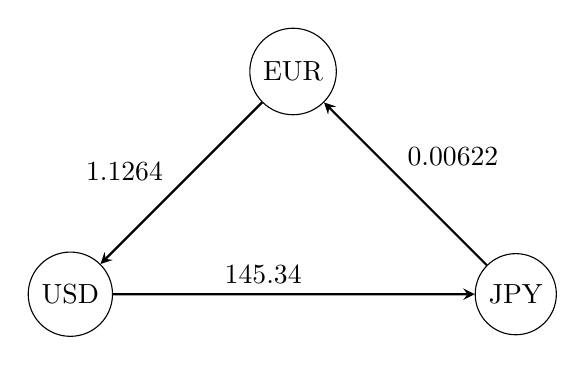
\begin{tikzpicture}[node distance=4cm, scale=0.7]
        \node (EUR) [draw, shape=circle] {EUR};
        \node (USD) [below left of=EUR, draw, shape=circle] {USD};
        \node (JPY) [below right of=EUR, draw, shape=circle] {JPY};

        \draw [arrow] (EUR) -- node[pos=0.55, above left] {$1.1264$} (USD);
        \draw [arrow] (USD) -- node[pos=0.55, above left] {$145.34$} (JPY);
        \draw [arrow] (JPY) -- node[pos=0.55, above right] {$0.00622$} (EUR);
    \end{tikzpicture}}
\end{figure}

In the above example, you can roundrip from one dollar to $145.34\times0.00622\times1.1264=\$1.0183$. If we scale the network, potential arbitrages won't be as obvious and we need an efficient algorithmic way to exploit them.

To scan such a graph for arbitrage opportunities, we won't go through the $\approx n!$ paths possible, but rather focus on finding interesting cycles.

\textit{Bellman-Ford} algorithm finds negative-weight cycles in time complexity $O(\lvert V \rvert \cdot \lvert E \rvert)$ by repeatedly relaxing the edges. We just need to transform the edges weights noticing that 
\begin{equation*}
    \resizebox{\hsize}{!}{$\text{USDJPY} \times \text{JPYEUR} \times \text{EURUSD} > 1 \Leftrightarrow -\log(\text{USDJPY}) -\log(\text{JPYEUR}) -\log(\text{EURUSD}) < 0.$}
\end{equation*}

One can also use \textit{Floyd-Warshall} which relies on dynamic programming\footnote{Shortest Path Faster Algorithm that blends Bellman-Ford and breadth-first search ideas (see this SPFA \href{https://konaeakira.github.io/posts/using-the-shortest-path-faster-algorithm-to-find-negative-cycles.html}{implementation}), while some other solutions use a divide-and-conquer approch \cite{yamada2002finding}; however we do not use Dijkstra as we can have edges with negative weights. Techniques from Kruskal's algorithm using union-find would work on an undirected graph, which is not the case here.}.

\begin{table}[h!]
    \centering
    \begin{tabular}{|c|c|c|}
        \hline
        \textbf{Algorithm} & \textbf{Time Complexity} & \textbf{Space Complexity} \\
        \hline
        Bellman-Ford & $O(|V| \cdot |E|)$ & $O(|V|)$ \\
        \hline
        Floyd-Warshall & $O(|V|^3)$ & $O(|V|^2)$ \\
        \hline
    \end{tabular}
    \caption{Algorithms to find negative-weight cycles}
    \label{tab:neg_cycle_algos}
\end{table}

\paragraph*{Going further} we could add bid and ask data, as well as factoring in transaction fees and liquidity constraints.